\chapter{JUNO}
%*prendo roba da JUno physics and detecto
%\section{Locazione e obiettivi generali}%magari scrivo qualcosina in più
Il Jiangmen Underground Neutrino Observatory (JUNO) \cite{JUNO:2021vlw} è un esperimento progettato a partire dal 2008 con l'obiettivo principale di determinare l'ordinamento di massa dei neutrini con significatività statistica di $3$ $-$ $4\,\,\sigma$ nel corso di sette anni di raccolta dati. Situato in Cina, grazie alla sua eccezionale risoluzione energetica e all'importante massa del rivelatore, JUNO ha diversi obiettivi tra cui la determinazione dei parametri di oscillazione $\sin^2{\theta_{12}}$, $\Delta m_{21}^2$ e $|\Delta m_{32}|^2$ con una precisione attesa al di sotto del $1\%$. Questi risultati saranno ottenuti principalmente attraverso la rivelazione di antineutrini elettronici provenienti da due reattori nucleari situati nella provincia di Guangdong, nel sud della Cina. Il rivelatore è infatti collocato a una distanza di circa $53\,\unit{km}$ da due grandi centrali nucleari: Yangjiang e Taishan. 

Oltre alla rivelazione degli antineutrini da reattore nucleare, JUNO sarà sensibile anche a neutrini provenienti da altre sorgenti naturali, come descritto nel capitolo precedente.

Al momento della stesura di questa tesi, JUNO ha completato la fase di riempimento con acqua, iniziata il 15 dicembre 2024. Successivamente, l'8 febbraio 2025, ha avuto inizio il riempimento con lo scintillatore liquido, fase in cui è stata raccolta la maggior parte dei dati da me analizzati.%come posso modificarla? Uso il presente o il passato?
\section{Struttura del rivelatore}
\begin{figure}[ht]
    %Sub-percent precision measurement of neutrino oscillation parameters with JUNO
    \centering
    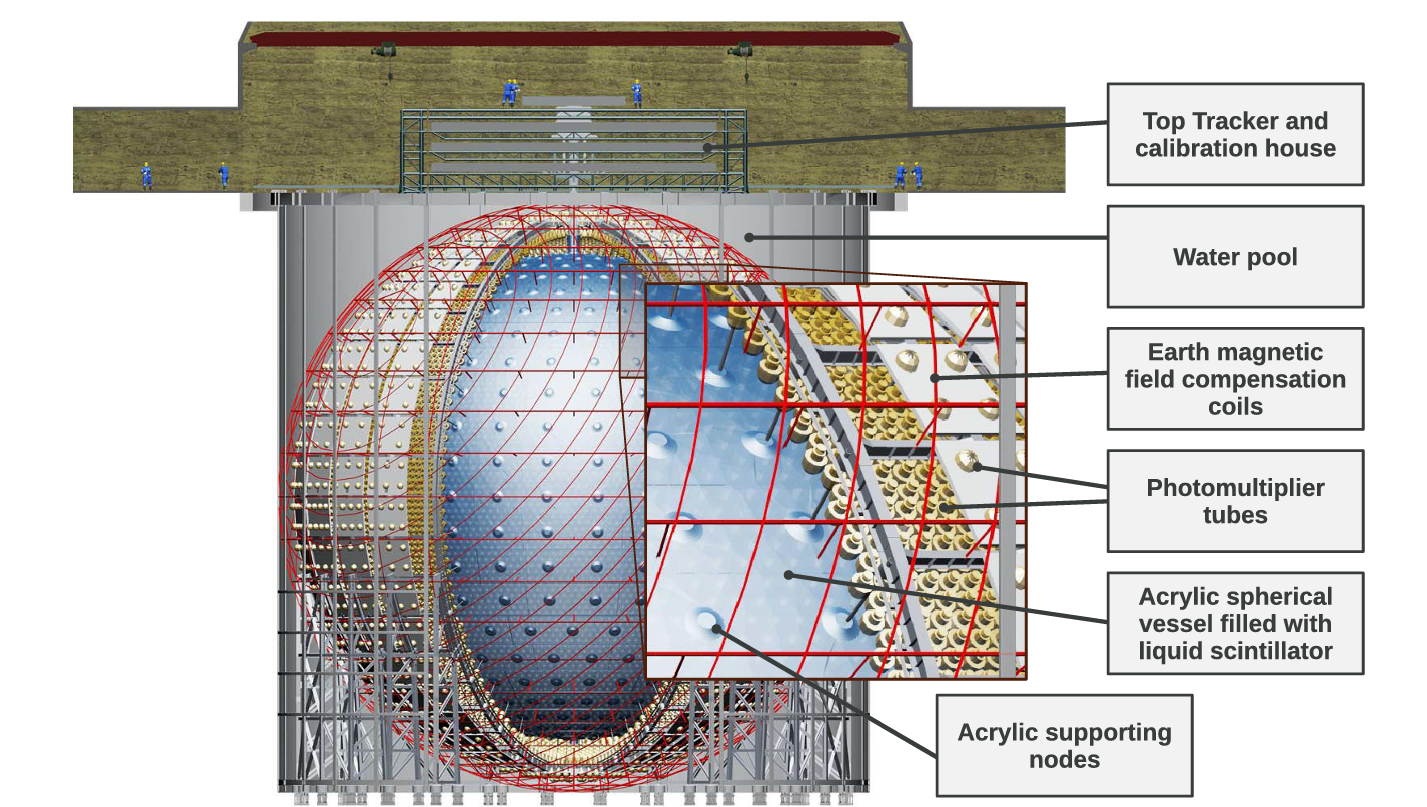
\includegraphics[width=1\textwidth]{Immagini/JUNO.png}
    \caption{Schema delle componenti principali di JUNO. Il diametro interno del Central Detector è di $35.4\,\unit{m}$ mentre il diametro della struttura in acciaio inossidabile in cui sono posizionati i PMT della Water Pool è di $40.1\,\unit{m}$ \cite{JUNO:2022mxj}.}
    \label{Fig:JUNO}
\end{figure}
%juno conceptual design report
JUNO si trova sotto una montagna di granito con un livello di copertura di roccia di $700\,\unit{m}$. Come è possibile osservare schematicamente dalla Figura \ref{Fig:JUNO} l'esperimento è composto da un rivelatore centrale (CD), un rivelatore Cherenkov ad acqua (Water Pool WP) e un tracker di muoni Top Tracker (TT). Di fondamentale importanza per gli obiettivi scientifici sono lo scintillatore liquido (LS) e i fotomoltiplicatori (PMT).
\vspace{0,5cm}
%miei appunti +  JUNOphysicsanddetector + JUNO Conceptual Design Report 74 75

\textbf{Scintillatore liquido organico}\\%rivedere la quantità di informazioni ma direi che ci siamo
Il principio di funzionamento dei rivelatori a scintillazione per rilevare radiazioni ionizzanti si basa sulla capacità di alcuni materiali di trasformare parte dell'energia assorbita dalla radiazione ionizzante in fotoni. L'efficienza di conversione della radiazione in luce, nota come light yield, è definita dal numero di fotoni prodotti per unità di energia rilasciata dalla radiazione incidente nel mezzo.

Gli scintillatori organici sono costituiti da idrocarburi aromatici, composti chimici contenenti anelli benzenici. La caratteristica principale di queste molecole è la presenza di orbitali ibridizzati. Nell'anello benzenico, gli orbitali $p$ si ibridizzano generando una banda di orbitali $\pi$. Quando una radiazione ionizzante interagisce con il materiale, può ionizzare gli atomi e portare gli elettroni in stati non legati. La successiva ricombinazione degli ioni può avvenire in due configurazioni energetiche: stati di singoletto o stati di tripletto.

Le transizioni interne degli stati di singoletto conducono a livelli eccitati che decadono verso lo stato fondamentale emettendo fotoni per fluorescenza. Uno scintillatore organico liquido viene preparato utilizzando un solvente in cui viene aggiunto in piccola quantità uno scintillatore efficiente detto fluoro: l'energia delle particelle viene trasferita dalle molecole del solvente a quelle del fluoro che emettono quindi luce. Inoltre, è molto importante anche la presenza di un secondo fluoro, detto wavelength-shifter: il suo compito è quello di assorbire la radiazione emessa del fluoro primario e riemetterla a lunghezze d'onda maggiori. Questo permette anche di effettuare il cosidetto matching tra i fotoni, emessi dallo scintillatore, e la risposta spettrale del fotocatodo dei PMT. In aggiunta, l'aumento della lunghezza d'onda dei fotoni serve ad evitare l'autossorbimento: se la radiazione emessa avesse una lunghezza d'onda compatibile con le transizioni molecolari del solvente, i fotoni verrebbero assorbiti rapidamente, rendendo lo scintillatore opaco ai suoi stessi fotoni.

Lo scintillatore liquido utilizzato da JUNO è una miscela ottimizzata composta da tre principali componenti:
%riguardare bene tutte le singole funzioni delle componenti
\begin{itemize}
    \item Solvente principale: il LAB (Linear Alkyl Benzene), un composto organico che costituisce la maggior parte del materiale bersaglio. Il LAB è responsabile dell'assorbimento dell'energia depositata dalle particelle ionizzanti con una prima emissione di luce con lunghezze d'onda minori.
    \item Fluoro primario: il PPO (2,5-difenilossazolo), in concentrazione di $2.5\,\unit{g/L}$.
    \item Wavelenght-shifter: il bis-MSB (1,4-bis(2-metil-stiril)-benzene), in concentrazione di $3\,\unit{mg/L}$. Questo componente, insieme al PPO, modifica la lunghezza d'onda dei fotoni emessi, portandola a circa $430\,\unit{nm}$. Questa risulta essere una regione ottimale per la sensibilità spettrale del fotocatodo dei PMT e rappresenta la lunghezza d'onda al di fuori dallo spettro di assorbimento, sia del solvente, sia del fluoro primario stesso.
\end{itemize}
\vspace{0,5cm}


\textbf{Tubi fotomoltiplicatori}\\
All'interno di JUNO sono presenti due tipi di fotomoltiplicatori. Il fotomoltiplicatore, mostrato schematicamente nella Figura \ref{Fig:PMT} a titolo di esempio nel caso di amplificazione a dinodi, è un tubo a vuoto in cui gli elettroni sono prodotti per effetto fotoelettrico. I fotoni emessi dalla parte liquida del rivelatore (LS o acqua) colpiscono il cosidetto fotocatodo producendo al più un elettrone per fotone. In generale un fotocatodo emette in media meno elettroni dei fotoni incidenti perchè non tutti i fotoni causano effetto fotoelettrico. Il rapporto tra elettroni prodotti e fotoni incidenti è detta efficienza quantica (quantum efficiency) \ref{eq:qe} del fotomoltiplicatore, che dipende dalla lunghezza d'onda incidente.
\begin{equation}
    QE(\lambda)=\frac{N_e}{N_\gamma(\lambda)}
    \label{eq:qe}
\end{equation}
Gli elettroni così prodotti sono accelerati da un campo elettrico, raggiungendo un'energia dell'ordine $\Delta V\approx10-100\,\unit{eV}$ e colpiscono un elettrodo, detto primo dinodo. Gli elettroni a queste energie estraggono altri elettroni dal metallo colpito, con un guadagno tra due e dieci elettroni per ogni elettrone incidente. Il processo si ripete tra il primo e il secondo dinodo, anche lui posto alla stessa differenza di potenziale rispetto al primo, innescando un effetto a cascata fino all'ultimo dinodo. La tensione è fornita tramite un generatore di tensione e, grazie ad un partitore resistivo, la tensione viene ripartita tra i dinodi. Il guadagno è funzione della tensione applicata e dal materiale di cui sono ricoperti i dinodi. Un altro parametro fondamentale per tutti i PMT è la cosiddetta dark current: il fotocatodo emette elettroni anche se non illuminato direttamente da luce, per effetto di temperatura e per estrazione dovuta alla presenza di un campo elettrico. Come conseguenza non tutti i fotoelettroni osservati sono dovuti all'interazione di particelle nel rivelatore.

L'obiettivo di JUNO di raggiungere una risoluzione energetica del $3\%$ al $\unit{MeV}$ richiede dei precisi requisiti costruttivi per i PMT impiegati. %magari qui posso mettere alcune caratteristiche di Juno che non ho trovato in nessun articolo
\begin{figure}[ht]
    %JUNOphysicsanddetector

    \centering
    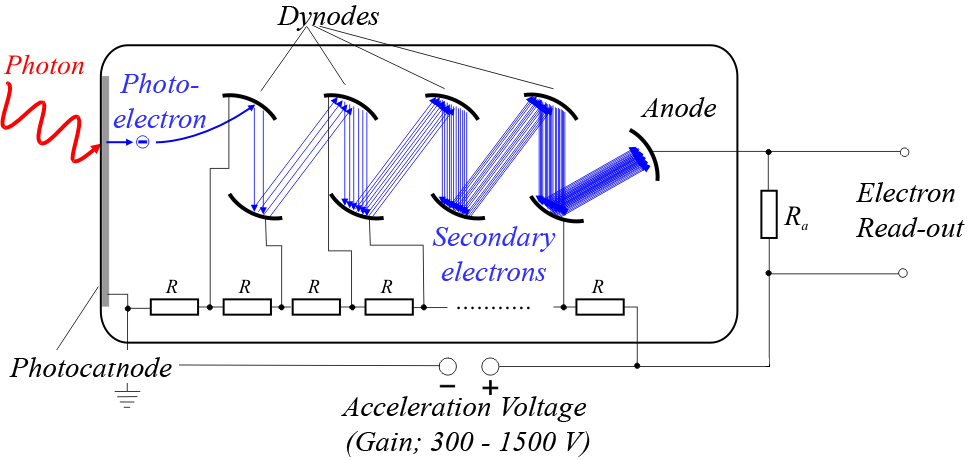
\includegraphics[width=0.8\textwidth]{Immagini/Photomultiplier_schema_en.png}
    \caption{Rappresentazione esemplificativa del funzionamento di un PMT con le componenti principali.}
    \label{Fig:PMT}
\end{figure}
\vspace{0,5cm}

\textbf{Il Rivelatore Centrale}\\
Il rivelatore centrale è una sfera in acrilico dal diametro interno di $35.4\,\unit{m}$ e spessore $12\,\unit{cm}$ che contiene $\sim20\,\unit{kton}$ di scintillatore liquido. Il CD è sorretto da una struttura in acciaio inossidabile in cui è installato un sistema di tubi fotomoltiplicatori: $17612$ PMT con diametro $50.8\,\unit{cm}$ (identificati come "large PMT") e $25600$ PMT con diametro $7.62\,\unit{cm}$ (identificati come ''small PMT''). Il sistema di tubi fotomoltiplicatori fornisce una copertura superficiale totale del $\sim78\%$.
%: i large PMT riescono a coprire il $75.2\%$ mentre i small PMT il $2.7\%$. 
 La struttura in acciaio inossidabile con un diametro di $40.1\,\unit{m}$, oltre a sostenere la sfera in acrilico e ospitare il sistema di tubi fotomoltiplicatori, contiene anche delle bobine al fine di compensare il campo magnetico terrestre che potrebbe peggiorare l'amplificazione del segnale dei fototubi. 
La sfera in acrilico è separata dai PMT attraverso un tampone d'acqua di spessore $1.42 \,\unit{m}$ che protegge il LS dalla radioattività del vetro dei PMT.

Per raggiungere gli obiettivi posti, è necessario che tutti i materiali che compongono il rivelatore centrale siano estremamente radiopuri e compatibili con il liquido scintillante e l'acqua.
\vspace{0,5cm}

\textbf{La Water Pool e il Top Tracker}\\%forse dovrei creare una sezione a parte in cui spiego nel dettaglio come funziona un rivelatore cherenkov, come avviene il traking dei muoni, e tutto il resto. O forse lascio così come è visto che questa è solo una sezione in cui spiego la struttura. Poi il funzionamenteo e le cose più dettagliate le descrivo in una sezione a parte
L'esperimento è composto da due sistemi di veto che forniscono un'efficiente riduzione del fondo dovuto agli isotopi cosmogenici indotti dal residuo del flusso di muoni cosmici che attraversano il rivelatore.
A far parte del sistema di veto di JUNO sono: il rivelatore ad acqua Cherenkov (WCD) e il Top Tracker (TT). Entrambi i sistemi collaborano per fornire un tracciamento attivo dei muoni cosmici. Come si può osservare dalla Figura \ref{Fig:JUNO}, il CD è immerso nel WCD che è un cilindro che contiene $35\,\unit{kton}$ di acqua ultra pura. Il cilindro ha un diametro di $43.5\,\unit{m}$ e un'altezza di $44\,\unit{m}$. Nella struttura in acciaio inossidabile del CD sono presenti $2400$ PMT rivolti verso l'esterno per misurare la luce Cherenkov emessa dalle particelle (muoni) che interagiscono in acqua. Il principale obiettivo del rivelatore ad acqua Cherenkov è di rivelare i muoni cosmici con una efficienza media del $99.5\%$. Oltre a questo, il WCD è di fondamentale importanza per schermare parte della radioattività esterna, mantenere la temperatura all'interno costante e fornire un supporto meccanico al CD.

Il Top Tracker è invece collocato al di sopra del WCD, come mostrato nella Figura \ref{Fig:TT}, è composto da $64$ ''TT walls'', ognuno composto da $512$ strisce di scintillatore plastico utilizzato nell'esperimento OPERA ai LNGS come Target Tracker. I TT walls sono distribuiti su tre strati in una griglia orizzontale $3\times7$, che copre un'area corrispondente al $25\%$ della superfice superiore del WCD. L'efficienza di ricostruzione del passaggio del muone è del $93\%$ con una risoluzione angolare di $0.20^\circ$. Il lavoro coordinato tra il top tracker, il WCD e il CD fornisce una buona ricostruzione del tracciato del muone e della produzione di isotopi cosmogenici all'esterno e all'interno del CD. Quest'ultimo è di fondamentale importanza per ottimizzare i diversi parametri di veto per i muoni da raggi cosmici.%che dici riscriviamo meglio? Lo cito solo perchè sto parlando della struttura. se la mia tesi si concentrerà anche su questo magari approfondicsco meglio.
\begin{figure}[ht]
    %JUNOphysicsanddetector

    \centering
    
\includegraphics[width=0.9\textwidth]{Immagini/tt.png}
    \caption{Il Top Tracker di JUNO è composto da una griglia $3\times7$ divisa in tre strati di scintillatori plastici e copre il $25\%$ della superficie del WCD \cite{JUNO:2021vlw}.}
    \label{Fig:TT}
\end{figure}
\section{Obiettivi scientifici}
L'obiettivo primario di JUNO è determinare l'ordinamento di massa dei neutrini (NMO). Come già introdotto nel primo capitolo, il problema dell'ordinamento di massa dei neutrini è determinato dalla mancata conoscenza del segno di $\Delta m_{3\ell}$, portando alla formazione di un ordinamento normale (NO, $m_1<m_2<m_3$) e ordinamento inverso (IO, $m_3<m_1<m_2$), come illustrato nella Figura \ref{Fig:Ordinamento}. JUNO sarà in grado di determinare l'ordinamento delle masse dei neutrini principalmente attraverso la misurazione del flusso di antineutrini elettronici provenienti dalle due centrali nucleari (Yangjiang e
Taishan) analizzando il pattern di interferenza nello spettro indotto dalle differenze di massa. La reazione di rivelazione utilizzata in questo caso è la reazione $\beta$ inversa \ref{eq:Beta inverso}. La distanza tra le centrali nucleari è stata decisa in maniera tale da massimizzare la differenza tra la probabilità di sopravvivenza in caso di ordinamento normale o inverso. Infatti ad una distanza di $\sim53\,\unit{km}$, JUNO misurerà simultaneamente oscillazioni guidate da piccoli splitting di massa ($\Delta m_{21}^2$) e grandi splitting di massa ($\Delta m_{31}^2$ e $\Delta m_{32}^2$), come mostrato nella Figura \ref{Fig:osc}.
\begin{figure}[ht]
    \centering
    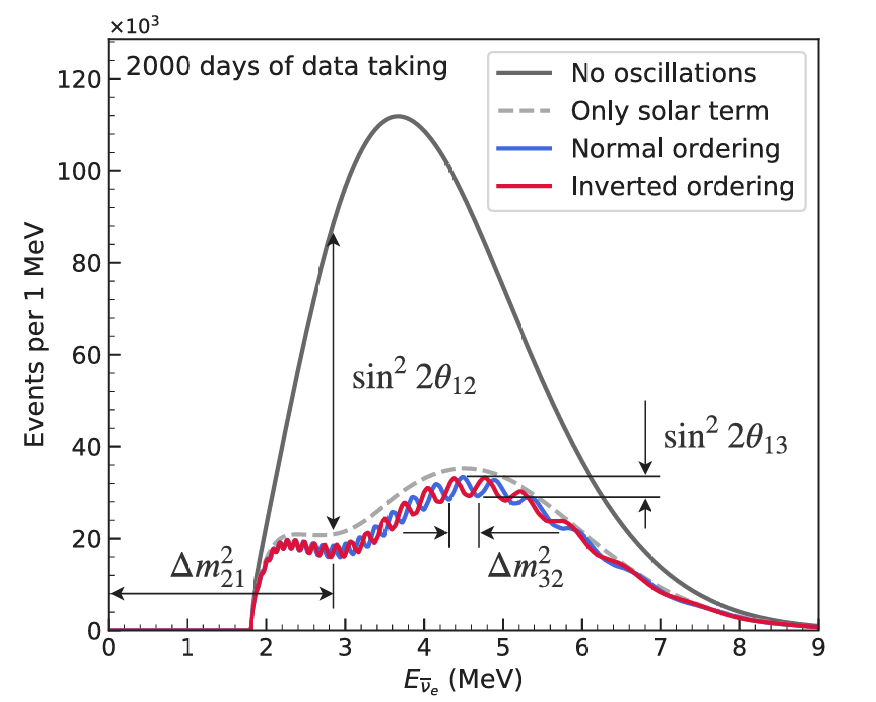
\includegraphics[width=0.6\textwidth]{Immagini/spettroenergia.png}
    \caption{Spettri energetici degli antineutrini da reattore attesi in 2000 giorni di presa dati. In grigio sono riportati gli eventi previsti in assenza di oscillazione, mentre in rosso e in blu sono mostrati gli eventi considerando rispettivamente l'ordinamento di massa inverso e normale. Viene inoltre mostrata la dipendenza dei quattro parametri di oscillazione \cite{JUNO:2021vlw}.}
    \label{Fig:osc}
\end{figure}

Oltre all'ordinamento delle masse dei neutrini, l'ampio volume fiduciale e l'eccellente risoluzione energetica di JUNO offrono ulteriori opportunità per affrontare importanti temi nella fisica dei neutrini, delle astro-particelle e della fisica solare.
\begin{itemize}
    \item \textbf{Neutrini da supernova:} rivelare neutrini di questo tipo è di fondamentale importanza per migliorare la comprensione dei meccanismi fisici che regolano le esplosioni stellari. Si stima che eventi di supernova nella Via Lattea avvengano ogni $30$-$40$ anni.  Di conseguenza, durante il periodo operativo di JUNO, c'è una significativa probabilità di osservare un simile evento, fornendo dati senza precedenti per lo studio della fisica delle supernove.
    \item \textbf{Diffuse supernova neutrino background (DSNB):} sebbene le supernove siano eventi relativamente rari nella nostra galassia, si verificano frequentemente nell'Universo visibile, generando un flusso diffuso di neutrini ($\sim10\,\nu\,\unit{cm^{-2}s^{-1}}$) che raggiunge in modo isotropo la Terra. Questo flusso, noto come DSNB, non è mai stato rivelato, ma si prevede che JUNO possa fornire evidenza della sua esistenza con significatività statistica di $3\sigma$ dopo $10$ anni di raccolta dati.
    \item \textbf{Geoneutrini:} sono antineutrini elettronici prodotti dal decadimento di isotopi radioattivi a vita media lunga, come quelli presenti nella catena di $\ce{^{238}U}$ e $\ce{^{232}Th}$, presenti all'interno della Terra. Questi rappresentano uno strumento per indagare il contributo del calore radiogenico della Terra. I geoneutrini sono rivelati da JUNO attraverso la reazione IBD \ref{eq:Beta inverso}.
    \item \textbf{Neutrini atmosferici:} grazie all'ampio volume del rivelatore e alla lunga esposizione, JUNO raccoglierà una grande quantità di dati sui neutrini atmosferici. Questi neutrini, prodotti dall'interazione dei raggi cosmici con l'atmosfera terrestre, contribuiscono alla determinazione dell'ordinamento di massa dei neutrini attraverso un'analisi indipendente dai dati forniti dagli antineutrini elettronici provenienti dai due centrali nucleari. Inoltre, l'elevata statistica e l'ottima risoluzione energetica di JUNO permetteranno uno studio dettagliato dell'angolo di mixing $\theta_{23}$ contribuendo a comprendere l'ottante in cui si colloca.
\end{itemize}
Tra i molteplici obiettivi scientifici di JUNO, lo studio dei neutrini solari riveste un ruolo centrale nel lavoro di questa tesi.  Attraverso l'analisi dei neutrini solari, sarà possibile approfondire sia le proprietà fondamentali dei neutrini stessi sia la struttura e la composizione chimica del Sole.
\section{Misura di neutrini solari}
%sto prendendo da Juno Physocs and detector ma da riguradare perchè non mi convince
I neutrini solari sono prodotti nel nucleo del Sole dai processi di fusione nucleare e rappresentano una sorgente naturale di neutrini fino a $16\,\unit{MeV}$. Come descritto nella sezione \ref{sec:sole}, lo studio di questi neutrini può fornire tantissime informazioni sulle proprietà della nostra stella e sui neutrini stessi. 

Anche se non sarà possibile raggiungere livelli di radiopurezza di altri esperimenti, come ad esempio Borexino, progettato in modo specifico per misurare i flussi di neutrini solari, JUNO compensa con la sua importante massa e ottima risoluzione energetica. Per questo motivo è un ottimo candidato per misurare i flussi di neutrini da reazione $\ce{^8B}$ ma anche da reazione $pep$, $\ce{^7Be}$ e da ciclo $\ce{CNO}$ fondamentali per i seguenti motivi:
\begin{itemize}
    \item \textbf{Il problema della Metallicità Solare}: la metallicità rappresenta la frazione di elementi chimici più pesanti dell'idrogeno e dell'elio presenti in una stella. La composizione chimica del Sole è un parametro chiave per la comprensione della struttura stellare e per lo sviluppo di modelli astrofisici accurati. Il problema della metallicità nasce dal disaccordo tra le previsioni del Modello Solare Standard e i dati dell'eliosismologia. Misure più precise del flusso di neutrini $\ce{^8B}$, $\ce{^7Be}$ e da ciclo $\ce{CNO}$ potrebbero contribuire a risolvere questa discrepanza.
    \item \textbf{Studio delle oscillazioni}: l'effetto Mikheyev-Smirnov-Wolfenstein (MSW) descrive come l'oscillazione del neutrino viene modificata dalla presenza di materia. Questa teoria prevede una transizione continua nella probabilità di sopravvivenza dei neutrini elettronici solari $P_{ee}$ quando l'energia passa da un range energetico alto, in cui domina l'effetto MSW, a basso in cui domina l'effetto vuoto. A causa delle difficoltà legate alla soglia energetica presentata dalla reazione ES (\ref{eq:scattel}) di circa $3.5\,\unit{MeV}$, la regione a bassa energia di transizione $P_{ee}$ non è ancora del tutto esplorata. Questa regione è di particolare interesse poiché alcuni modelli teorici suggeriscono che potrebbe essere sensibile a interazioni oltre il Modello Standard nel canale dello scattering elastico neutrino-elettrone.
    \item \textbf{Studio dei parametri di oscillazione}: le future misurazioni ad alta precisione di $\sin^2{\theta_{12}}$ e $\Delta m^2_{21}$, basate sui neutrini solari, potranno essere utilizzate per testare la coerenza della struttura standard dei tre neutrini e per sondare la nuova fisica oltre il Modello Standard.
\end{itemize}
%voglio dire che sono quelli più abbondanti e di conseguenza rispetto ad altri processi di produzione dei neutrini corrispondono ad una quantità più piccola rispetto a quelli da 8B

%in futuro magari posso aggiungere una sezione in cui parlo di questo effetto
\section{Fondi radioattivi}
\label{sec:fondi}
Un aspetto essenziale per lo studio dell'ordinamento di massa del neutrino e del flusso di neutrini solari \cite{JUNO:2020hqc} riguarda il background causato dai fondi radioattivi. Nel caso della rivelazione di antineutrini elettronici, il passaggio dei muoni cosmici attraverso il rivelatore innesca processi di spallazione, generando isotopi emettitori di $\beta$-neutroni e neutroni veloci, prodotti anche dall'interazione dei muoni con la roccia circostante. Questi fenomeni costituiscono un potenziale fondo per il segnale di IBD \ref{eq:Beta inverso}, il processo utilizzato per la rivelazione di $\bar{\nu}_e$. Tuttavia, il loro contributo può essere significativamente ridotto grazie a un sistema di veto basato sulla ricostruzione della traccia del muone e su una selezione accurata del volume fiduciale (FV). 

Il sistema di doppio veto per i muoni, composto dal Top Tracker e dal rivelatore Cherenkov ad acqua, garantisce un'alta efficienza nella marcatura dei muoni, permettendo di ridurre efficacemente il fondo cosmogenico. La strategia di veto ottimizzata per ottenere un rapporto fondo/segnale inferiore al $3\%$ si basa principalmente sulla ricostruzione della traccia del muone. 

Nel caso della misura del flusso di neutrini solari, la presenza di fondo radioattivo è un aspetto cruciale da considerare. In particolare, lo scattering elastico con gli elettroni, essendo un segnale singolo, non presenta eventi correlati che possano essere utilizzati per sopprimere il background durante le misure. Il background può essere classificato come interno ed esterno e dovuto dai muoni che indicono neutroni e isotopi cosmogenici.
\vspace{0,2cm}

\textbf{Radioattività interna}\\
La radioattività interna costituisce un fondo di misura legato all'ineliminabile contaminazione del LS, presente in quantità ridotte. I requisiti minimi di radiopurezza per l'obiettivo di determinazione NMO impone una soglia di contaminazione inferiore di $10^{-15}\,\unit{g/g}$ per gli isotopi appartenenti alle catene del $\ce{^238U}$ e $\ce{^232Th}$. Data la soglia ineliminabile di reazione bisogna, considerare solamente gli eventi al di sopra di $2\,\unit{MeV}$. Oltre alla possibile contaminazione ignota da $\ce{^{238}U}/\ce{^{232}Th}$ esistono altri isotopi radioattivi che però non influiscono l'analisi in quanto il Q valore è al di sotto della soglia intrinseca come è possibile osservare a destra nella Figura \ref{Fig:inter}.
\begin{figure}[ht]
    \centering

    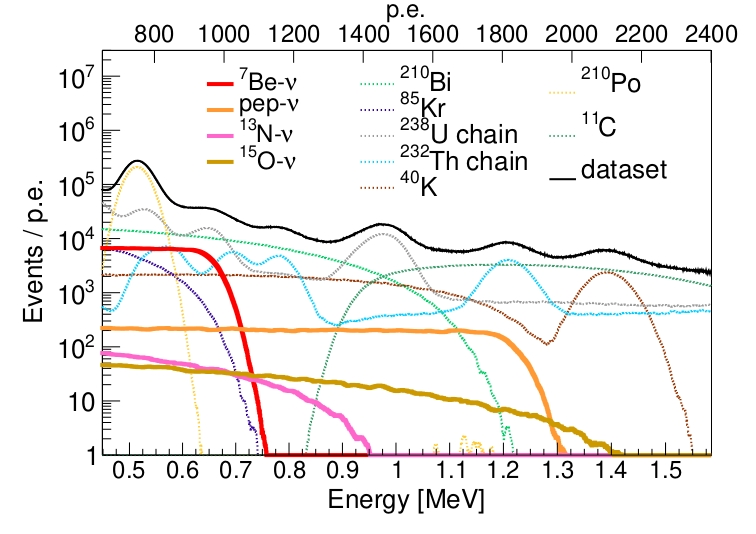
\includegraphics[width=0.49\textwidth]{Immagini/fodno.jpg}
    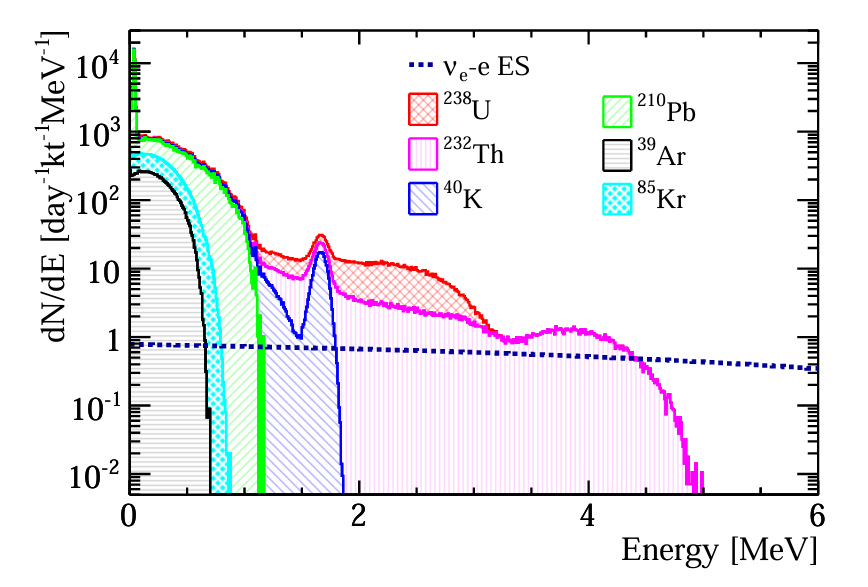
\includegraphics[width=0.49\textwidth]{Immagini/interno.png}
    \caption{A sinistra: contributi di neutrini e fondi radioattivi per l'analisi di sensibilità dei neutrini solari $\ce{^7Be}$, $pep$ e  $\ce{CNO}$ , simulati su sei anni di raccolta dati nello scenario di radiopurezza $10^{-16}\unit{g/g}$ per $\ce{^238U}$ e $\ce{^232Th}$. A destra: spettro energetico della radioattività del LS in JUNO.}
    \label{Fig:inter}
\end{figure}
%posso anche citare semplicemente che c'è un metodo per tagliare questo fondo e aggiungere di fianco il grafico dello spettro dopo il taglio. Solo per citarlo ecco.
\vspace{0,2cm}

\textbf{Radioattività esterna}\\
Grazie alla quantità d'acqua che separa il LS dalla roccia (almeno $3.5\,\unit{m}$ e in media $5\,\unit{m}$), il contributo della radioattività naturale esterna, come i raggi $\gamma$ e i neutroni radiogenici e cosmogenici nella roccia, è significativamente ridotto. Il rate di eventi associati a questi processi è limitato a circa $10\,\unit{Hz}$ sull'intero volume del LS. Il contributo primario al fondo esterno è dovuto alle parti in acciaio inossidabile della struttura che sorregge il CD, al vetro dei PMT e al radon presente in acqua. Selezionando via software un volume fiduciale (FV), cioè una porzione sferica di scintillatore in cui il rapporto segnale-rumore è massimizzato, il fondo esterno può essere ridotto come si può osservare dalla Figura \ref{Fig:est}. Ad esempio, selezionando una sfera di raggio $R =13\,\unit{m}$, il fondo esterno è ridotto a meno del $0.5\%$ comparato con i segnale di range energetico intorno a $2-3\,\unit{MeV}$ in cui rimangono $8\,\unit{kton}$ di target attivo.
\begin{figure}[ht]
    \centering
    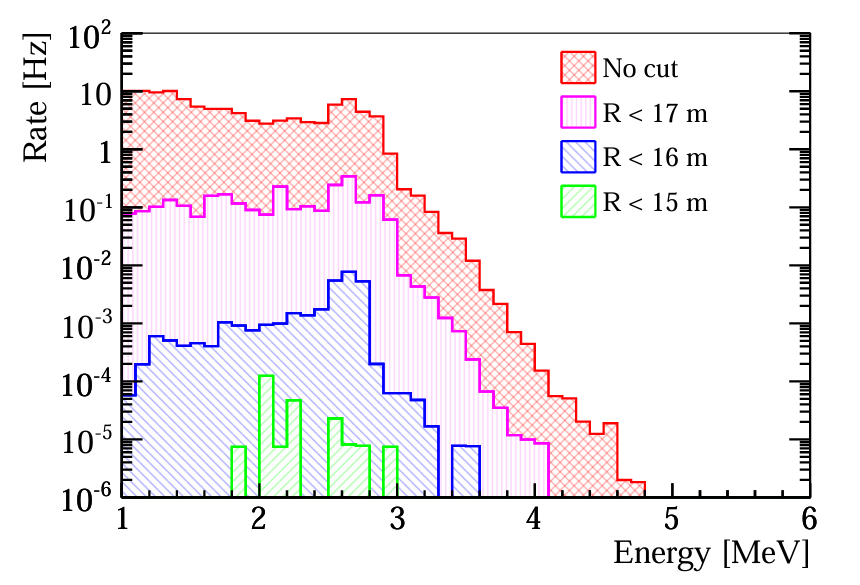
\includegraphics[width=0.56\textwidth]{Immagini/esterna.png}
    \caption{Spettro energetico atteso in JUNO per la radioattività esterna dopo selezioni di volume fiduciale come sfere di diverso raggio.}
    \label{Fig:est}
\end{figure}
Gli eventi con un'energia maggiore derivano dalla cattura neutronica dei materiali che compongono o circondano il rivelatore. I neutroni possono essere di natura radiogenica o cosmogenica. I primi derivano, ad esempio, dalla fissione spontanea di $\ce{^{238}U}$ in cui il neutrone può essere catturato portando il materiale in uno stato eccitato ed emettendo fotoni di energia variabile tra $8-10\,\unit{MeV}$. Questi, con un FV di $R<17\,\unit{m}$, sono completamente trascurabili.

\vspace{0,2cm}

\textbf{Isotopi e neutroni cosmogenici indotti da muoni}\\
Il rivelatore JUNO, pur avendo $\sim700\,\unit{m}$ di roccia soprastante, è bersagliato da un flusso residuo di muoni. Il flusso dei muoni è di circa $0.0037\,\unit{Hz/m^2}$ con un'energia media di $209\,\unit{GeV}$. Durante il loro passaggio, i muoni possono innescare processi di spallazione, generando isotopi radioattivi e neutroni veloci come descritto all'inzio di questa sezione. Nel range energetico inferiore a $1.5\,\unit{MeV}$, come è possibile ossevare a sinistra della Figura \ref{Fig:inter}, il principale fondo che ostacola la misura dei neutrini solari in particolare da ciclo $\ce{CNO}$ e $\ce{^7Be}$ è l'isotopo cosmogenico $\ce{^11C}$, caratterizzato da una vita media di circa $27 \unit{min}$. Allo stesso modo vengono sfruttate le medesime tecniche di veto basate sulla ricostruzione del tracciato dei muoni e sull'individuazione dei neutroni prodotti nelle interazioni secondarie, permettendo di ridurre in modo efficace il background cosmogenico.

La ricostruzione degli eventi candidati muoni rappresenta il tema centrale di questa tesi e sarà approfondita nel capitolo \ref{cap:muon}.
%vorrei collegarmi 
%non parlo del fondo dovuto agli antineutrini da reattore in quanto non serve.
\section{Il riempimento del rivelatore JUNO}
La fase di riempimento con acqua, iniziata il 15 dicembre 2024, è stata completata con successo. Durante questa fase, la Water Pool e il Central Detector sono stati riempiti contemporaneamente, permettendo di testare l'intero sistema dal punto di vista ingegneristico e di facilitare il successivo riempimento con lo scintillatore liquido. A seguito di questa fase, l'8 febbraio 2025 ha avuto inizio il riempimento con il LS nel CD.

Una volta che la Water Pool e il Central Detector sono stati riempiti completamente, è stato possibile iniziare la caratterizzazione del flusso di muoni incidenti nel rivelatore, sfruttando la loro elevata energia e i fotoni Cherenkov prodotti durante il loro passaggio nel rivelatore stesso. L'effetto Cherenkov è un fenomeno fisico che si verifica quando una particella carica interagisce con il mezzo e si propaga a una velocità superiore a quella della luce nel mezzo. Questo provoca l'emissione di fotoni che si propagano, secondo un cono con asse coincidente con la direzione della particella, fino a raggiungere i tubi fotomoltiplicatori, che li raccolgono e, grazie all'effetto fotoelettrico a cascata, produce una carica in fotoelettroni che genera un segnale rilevabile.

Il riempimento con LS è stimato durare circa 6-7 mesi, con una velocità di riempimento di 7 $\unit{m^3/h}$ di LS inseriti nel CD. Durante questa fase, la presa dati del rivelatore, sia per il CD che per la WP, è regolare, permettendo di iniziare a studiare gli eventi rivelati. Questo è utile per comprendere meglio la risposta del rivelatore e le problematiche connesse, sia dal punto di vista hardware (trigger, acquisizione dati, pre-selezione dei dati online) che software (accesso alle strutture dati, ricostruzione degli eventi).
Dal punto di vista delle analisi fisiche, lo studio della radioattività del liquido scintillatore è un tema chiave in questa fase. Inoltre, è possibile caratterizzare il flusso di muoni, che costituiscono la causa principale del background cosmogenico per tutte le future analisi. Come accennato nella sezione precedente, un'analisi dettagliata dei muoni è fondamentale per molte delle misure previste con JUNO, dai neutrini solari agli antineutrini elettronici da reattore.